\chapter{Multiplicidad, entropía y equilibrio con restricciones}

\lectureoverview{Una distribución de probabilidad se convierte en un objeto termodinámico cuando sus estados tienen energías. Primero relacionamos el aumento de la entropía con la equilibración y usamos \(dE=T\,dS\) para deducir el sentido del flujo de calor. Después sustituimos un sistema por un conjunto grande de réplicas, contamos las configuraciones asociadas a cada conjunto de números de ocupación y mostramos que el logaritmo de esta multiplicidad es igual a la entropía multiplicada por \(N\). El equilibrio es, por tanto, un problema de maximización de la entropía con restricciones. Los multiplicadores de Lagrange proporcionan el método necesario para resolverlo.}

\section{Las tres magnitudes básicas}

Sea \(i\) la etiqueta de los estados discretos disponibles para un sistema. Por ahora, la discreción resulta útil porque nos permite contar estados sin introducir medidas del espacio de fases. Si la probabilidad del estado \(i\) es \(P_i\), entonces
\begin{equation}
 \sum_i P_i=1.
 \label{eq:sm3-normalization}
\end{equation}
Si la energía de ese estado es \(E_i\), la energía media es
\begin{equation}
 \overline E=\sum_iP_iE_i.
 \label{eq:sm3-mean-energy}
\end{equation}
La palabra \emph{media} es importante. El sistema no tiene por qué poseer el valor \(\overline E\) en ningún estado microscópico; se trata del promedio ponderado por las probabilidades de los valores posibles.

\begin{classroomqa}
\classquestion{¿Hay aquí alguna distinción útil entre probabilidad y estadística?}
\lecturerresponse{La probabilidad proporciona un modelo de los resultados posibles, mientras que la estadística suele partir de datos observados y pregunta qué se puede inferir de ellos. En este cálculo usamos distribuciones de probabilidad, aunque los mismos promedios aparecen de manera natural en los datos estadísticos. En el intercambio informal de clase, las palabras se usan sin demasiado rigor porque esa distinción no afecta a la física que sigue.
\lecturetimestamp{00:01:39--00:02:21}}
\end{classroomqa}

La entropía de la distribución es
\begin{equation}
 S[P]=-\sum_iP_i\log P_i.
 \label{eq:sm3-entropy}
\end{equation}
Esta expresión es no negativa. Toda probabilidad no nula satisface \(0<P_i\leq1\), así que \(\log P_i\leq0\), y cuando \(P_i\to0\) se aplica el valor límite convencional \(P_i\log P_i\to0\).

\begin{figure}[t]
\centering
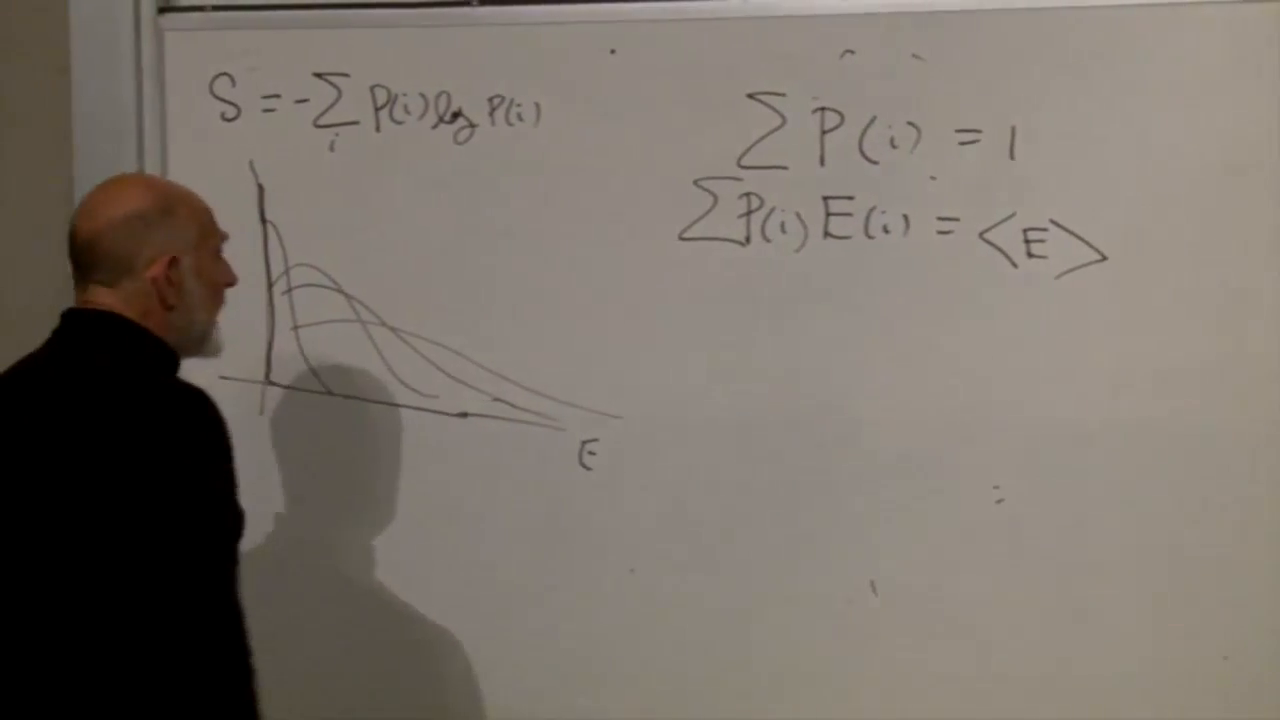
\includegraphics[width=0.88\textwidth]{lecture_03_figure_02.png}
\caption{La pizarra inicial reúne las fórmulas de la entropía, la normalización y la energía media, junto con una familia cualitativa de distribuciones de equilibrio.}
\lectureframe{00:06:44}
\end{figure}

\section{El equilibrio como familia de distribuciones}

La clase anterior nos dejó una familia de distribuciones de equilibrio con un parámetro. Se puede etiquetar esa familia mediante la temperatura, pero por ahora resulta más útil hacerlo mediante la energía media \(\overline E\). A la energía mínima posible, la distribución se concentra en un estado fundamental:
\[
 P_i=\delta_{i0}.
\]
En ese caso no hay incertidumbre sobre el estado y \(S=0\). A medida que la distribución de equilibrio se extiende por más niveles de energía, aumentan tanto su energía media como su entropía.

Esto es cierto para la familia térmica, no para cualquier distribución que se pueda imaginar. Una familia arbitraria podría desplazarse hacia energías mayores y, al mismo tiempo, estrecharse. Las distribuciones de equilibrio que deduciremos no se comportan así en el régimen habitual de temperatura positiva. A lo largo de esa familia,
\begin{equation}
 \frac{dS}{d\overline E}>0.
 \label{eq:sm3-positive-temperature-branch}
\end{equation}
Los sistemas con espectros acotados también pueden tener ramas en las que esta derivada es negativa. Esos regímenes de temperatura negativa son reales, pero los dejaremos de lado en el argumento presente.

El equilibrio térmico es algo más que la inmovilidad microscópica. Las moléculas siguen moviéndose, chocando e intercambiando energía. Lo que se vuelve estacionario es la descripción macroscópica: la distribución deja de presentar una deriva neta y las distintas partes del sistema dejan de mantener un flujo neto de energía.

\section{Las leyes de la termodinámica en lenguaje estadístico}

La primera ley expresa la conservación de la energía. La segunda ley establece que la entropía termodinámica de un sistema macroscópico aislado no disminuye:
\begin{equation}
 \Delta S_{\mathrm{tot}}\geq0.
 \label{eq:sm3-second-law}
\end{equation}
La igualdad describe el equilibrio o un cambio reversible ideal; una relajación espontánea suele producir un aumento estricto.

En el enfoque probabilístico, la relajación tiende a repartir el peso entre las alternativas macroscópicas que aún distinguimos. Esta afirmación requiere la precisión que se hizo en la clase: estamos haciendo un \emph{coarse-graining}. La evolución hamiltoniana exacta conserva la entropía del espacio de fases de grano fino. La entropía macroscópica aumenta porque dejamos de seguir las correlaciones y los detalles microscópicos. Al perder esa información, la descripción reducida se vuelve más amplia. Un estrechamiento espontáneo implicaría, en cambio, que hemos adquirido información microscópica sin realizar una medición.

La ley cero afirma que los sistemas pueden alcanzar el equilibrio térmico y que el equilibrio es transitivo. Si \(A\) está en equilibrio con \(B\), y \(B\) con \(C\), entonces \(A\) está en equilibrio con \(C\). La temperatura proporciona la magnitud que hace explícita esta transitividad:
\[
 T_A=T_B,\qquad T_B=T_C
 \quad\Longrightarrow\quad
 T_A=T_C.
\]
Fuera del equilibrio, la energía fluye del subsistema de mayor temperatura al de menor temperatura. Cuando las temperaturas son iguales, el flujo neto cesa. Ahora deduciremos esta afirmación operacional a partir de la definición de temperatura basada en la entropía.

\section{Por qué la energía fluye de caliente a frío}

Consideremos dos subsistemas débilmente acoplados, \(A\) y \(B\). Cada uno está en equilibrio interno, pero sus temperaturas son distintas. Elijamos las etiquetas de modo que
\begin{equation}
 T_B>T_A>0.
 \label{eq:sm3-temperature-order}
\end{equation}
Durante un pequeño intercambio, la conservación de la energía total da
\begin{equation}
 dE_A+dE_B=0.
 \label{eq:sm3-energy-conservation}
\end{equation}
La segunda ley establece que
\begin{equation}
 dS_A+dS_B\geq0.
 \label{eq:sm3-entropy-change}
\end{equation}
Para cada subsistema en equilibrio interno, la temperatura se define mediante
\begin{equation}
 dE_X=T_X\,dS_X,
 \qquad X=A,B.
 \label{eq:sm3-temperature-differential}
\end{equation}
Al sustituir en \eqref{eq:sm3-energy-conservation} se obtiene
\begin{equation}
 T_A\,dS_A+T_B\,dS_B=0,
\end{equation}
y, por tanto,
\begin{equation}
 dS_B=-\frac{T_A}{T_B}\,dS_A.
 \label{eq:sm3-dsb}
\end{equation}
Al introducir este resultado en \eqref{eq:sm3-entropy-change},
\begin{align}
 dS_{\mathrm{tot}}
 &=dS_A-\frac{T_A}{T_B}dS_A\\
 &=\frac{T_B-T_A}{T_B}\,dS_A\geq0.
 \label{eq:sm3-flow-entropy}
\end{align}
Como \(T_B-T_A>0\) y \(T_B>0\), un intercambio espontáneo requiere que
\[
 dS_A>0.
\]
Entonces, la ecuación \eqref{eq:sm3-temperature-differential} da
\begin{equation}
 dE_A=T_A\,dS_A>0,
 \qquad
 dE_B=-dE_A<0.
 \label{eq:sm3-hot-to-cold}
\end{equation}
La energía ha fluido desde \(B\), el subsistema más caliente, hacia \(A\), el más frío. Aquí, el calor no es más que energía en tránsito. El flujo continúa hasta que \(T_A=T_B\), cuando el cambio de entropía de primer orden deja de favorecer cualquiera de los dos sentidos.

El mismo resultado se puede expresar en una sola línea:
\begin{equation}
 dS_{\mathrm{tot}}
 =dE_A\left(\frac{1}{T_A}-\frac{1}{T_B}\right)\geq0.
 \label{eq:sm3-compact-flow}
\end{equation}
El signo de la diferencia de temperaturas inversas determina el signo de \(dE_A\). Esta forma compacta encajará de manera natural con el conjunto canónico más adelante.

\begin{classroomqa}
\audiencequestion{¿Este argumento supone que \(A\) y \(B\) ya están cada uno en equilibrio interno?}
\lecturerresponse{Sí. Asignar un único \(T_A\) o \(T_B\) implica ese supuesto. Si un subsistema no está en equilibrio interno, hay que dividirlo en regiones más pequeñas y aplicar localmente el argumento allí donde se pueda definir una temperatura. La relajación global se obtiene entonces a partir de los intercambios entre esas regiones.
\lecturetimestamp{00:24:38--00:25:22}}
\end{classroomqa}

\section{¿Qué cuenta como estado?}

Antes de preguntar cuáles son las probabilidades de equilibrio, debemos saber qué significa la etiqueta \(i\). Un estado microscópico es la especificación más completa del sistema que permiten las leyes físicas subyacentes. En mecánica clásica, se imagina que se dan las posiciones y los momentos de todas las partículas. En mecánica cuántica, en cambio, un estado es un estado cuántico completo; el principio de incertidumbre impide especificar simultáneamente con precisión todas las posiciones y momentos clásicos.

Para un sistema cuántico en una caja finita, el recuento pertinente de estados puede ser discreto. La mecánica estadística clásica surge en un límite apropiado, en el que las sumas sobre estados cuánticos muy próximos entre sí se convierten en integrales sobre el espacio de fases. Ese proceso límite también introduce la celda del espacio de fases necesaria para que la entropía continua sea adimensional; no se obtiene simplemente sustituyendo un signo de suma por uno de integral.

\begin{classroomqa}
\audiencequestion{Para un gas, ¿hay que imaginar un estado como las posiciones y los momentos de cada molécula?}
\lecturerresponse{Esa es la imagen clásica correcta. En general, un estado significa todo lo que, en principio, se podría conocer del sistema, de acuerdo con las leyes físicas. La mecánica cuántica modifica la forma de esa descripción máxima y hace discreto el recuento en un volumen finito. Recuperar la integral clásica a partir de la suma cuántica requiere un verdadero argumento de paso al límite, no una sustitución en una sola línea.
\lecturetimestamp{00:25:31--00:27:38}}
\end{classroomqa}

\section{Un baño térmico compuesto de réplicas}

Ahora ya no podemos eludir la pregunta difícil: una vez establecido el equilibrio, ¿qué determina \(P_i\)?

Pongamos el subsistema en contacto con un baño térmico muy grande. La energía puede pasar en ambos sentidos, pero el baño tiene tantos grados de libertad que la transferencia de una pequeña cantidad de energía apenas cambia su temperatura. Un baño especialmente conveniente consiste en muchas réplicas del propio subsistema, débilmente acopladas entre sí. Una réplica es el sistema que estudiamos; las demás constituyen su entorno.

Esta construcción suele reflejar un sistema macroscópico real. Dividamos un cuerpo grande y casi homogéneo en muchas celdas similares. Cada celda es un subsistema y las celdas restantes actúan como su baño. Denotemos por \(N\) el número total de réplicas. La demostración en clase usa nueve réplicas y tres etiquetas de estado de distintos colores, pero el recuento no depende de esos números concretos.

Sea \(n_i\) el número de réplicas en el estado \(i\). Estos son los \emph{números de ocupación}. Puede haber infinitos niveles de energía posibles, pero, a energía total finita, la ocupación de la mayoría de los niveles muy altos es despreciable o nula.

La primera restricción expresa simplemente el número de réplicas:
\begin{equation}
 \sum_i n_i=N.
 \label{eq:sm3-number-constraint}
\end{equation}
La segunda es la energía total:
\begin{equation}
 \sum_i n_iE_i=N\overline E.
 \label{eq:sm3-total-energy-constraint}
\end{equation}
El miembro derecho es extensivo. Si se duplica el número de réplicas manteniendo fijo su estado estadístico, se duplica la energía total, mientras que la energía media por réplica sigue siendo \(\overline E\).

\begin{classroomqa}
\audiencequestion{¿La construcción con réplicas también debe satisfacer una restricción de energía?}
\lecturerresponse{Sí. Los números de ocupación deben sumar \(N\), y su suma ponderada por la energía debe ser igual a la energía total fija \(N\overline E\). Esas son precisamente las dos restricciones que limitarán más adelante la maximización de la entropía.
\lecturetimestamp{00:37:12--00:39:54}}
\end{classroomqa}

La probabilidad de que una réplica elegida al azar ocupe el estado \(i\) es su frecuencia relativa:
\begin{equation}
 P_i=\frac{n_i}{N},
 \qquad
 n_i=NP_i.
 \label{eq:sm3-frequency-probability}
\end{equation}

\begin{figure}[t]
\centering
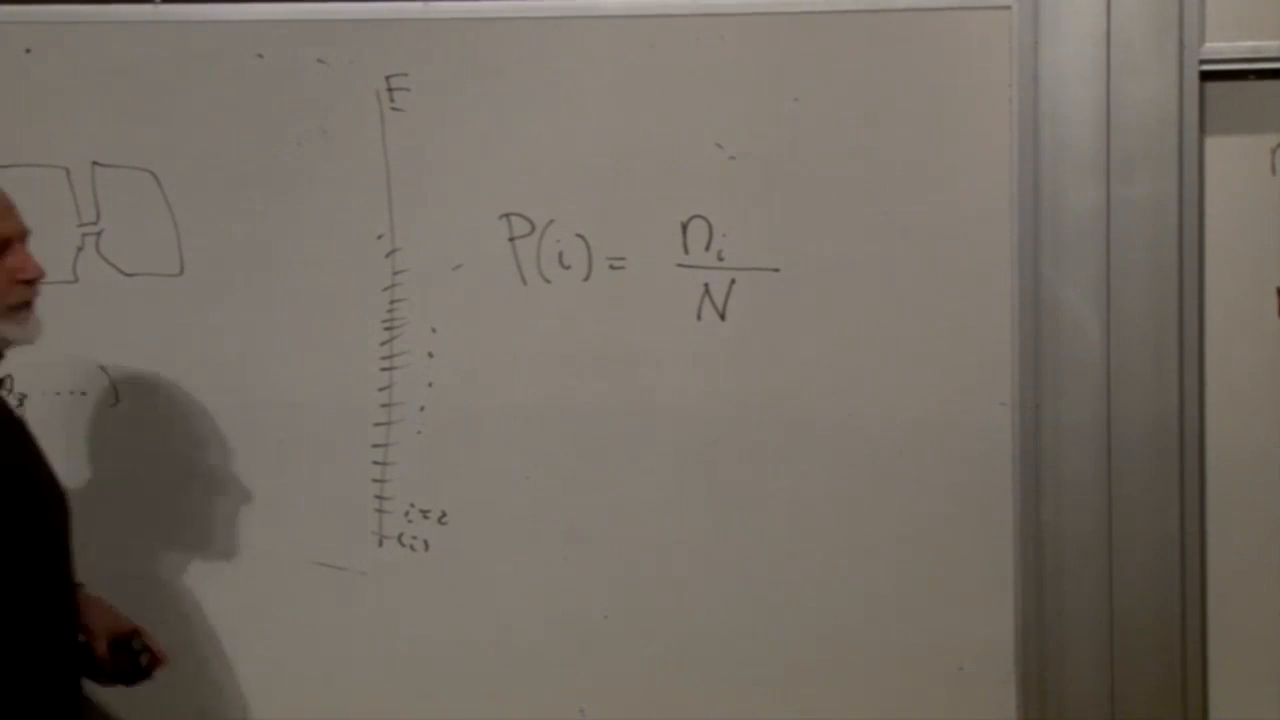
\includegraphics[width=0.82\textwidth]{lecture_03_figure_03.png}
\caption{La imagen de los niveles de energía y la identificación de la probabilidad con la fracción de ocupación \(P_i=n_i/N\).}
\lectureframe{00:41:40}
\end{figure}

\begin{classroomqa}
\audiencequestion{¿Se pretende que la notación \(N(i)\) de la pizarra sea distinta de \(n_i\)?}
\lecturerresponse{No. Ambas notaciones representan el número de ocupación del estado \(i\). Usaremos \(n_i\) de manera sistemática y reservaremos la mayúscula \(N\) para el número total de réplicas.
\lecturetimestamp{00:41:28--00:41:33}}
\end{classroomqa}

Al dividir \eqref{eq:sm3-number-constraint} y \eqref{eq:sm3-total-energy-constraint} entre \(N\) se recuperan las restricciones sobre las probabilidades:
\begin{equation}
 \sum_iP_i=1,
 \qquad
 \sum_iP_iE_i=\overline E.
 \label{eq:sm3-probability-constraints}
\end{equation}
La interpretación de las frecuencias en el conjunto ha reproducido, por tanto, las ecuaciones con las que empezamos.

\section{Multiplicidad de un patrón de ocupación}

Fijemos un conjunto de números de ocupación \(\{n_i\}\). ¿Cuántas asignaciones de las \(N\) réplicas distinguibles a los estados dan exactamente ese conjunto? La respuesta es el coeficiente multinomial
\begin{equation}
 C(\{n_i\})=\frac{N!}{\prod_i n_i!}.
 \label{eq:sm3-multiplicity}
\end{equation}
Para entender el denominador, primero ordenamos las \(N\) réplicas etiquetadas de \(N!\) maneras. Reordenar las \(n_i\) réplicas que ocupan el mismo estado no genera una nueva asignación de ocupación, así que dividimos por \(n_i!\) para cada estado.

\begin{figure}[t]
\centering
\includegraphics[width=0.88\textwidth]{lecture_03_figure_04.png}
\caption{La multiplicidad multinomial \(C=N!/\prod_i n_i!\) escrita en la pizarra.}
\lectureframe{00:46:55}
\end{figure}

Los niveles desocupados no plantean ningún problema porque \(0!=1\). Si todas las réplicas ocupan un mismo estado, entonces
\[
 C=\frac{N!}{N!}=1,
\]
como cabía esperar. Si tres réplicas ocupan tres estados especificados distintos, entonces
\[
 C=\frac{3!}{1!\,1!\,1!}=6.
\]
Cuando dos réplicas ocupan dos estados especificados, la fórmula da dos asignaciones: se intercambia cuál de las réplicas etiquetadas ocupa cada estado.

\begin{classroomqa}
\audiencequestion{¿Puede haber más de un conjunto de números de ocupación que satisfaga las dos restricciones?}
\lecturerresponse{Por lo general, sí, hay muchos. La ecuación \eqref{eq:sm3-multiplicity} cuenta primero las configuraciones para un conjunto fijo \(\{n_i\}\), sin decidir aún si satisface las restricciones. En la etapa siguiente se comparan todos los conjuntos compatibles con ellas y se encuentra cuál tiene la multiplicidad más grande.
\lecturetimestamp{00:48:07--00:48:43}}
\end{classroomqa}

El supuesto estadístico es que las asignaciones microscópicas compatibles con la configuración aislada se tratan simétricamente. Por tanto, un patrón macroscópico de ocupación que se realiza de más maneras es más probable. Cuando \(N\) es grande, la distribución de las fracciones \(n_i/N\) tiene un pico muy pronunciado. Las fracciones de equilibrio son los valores que maximizan \(C\), con las restricciones \eqref{eq:sm3-number-constraint} y \eqref{eq:sm3-total-energy-constraint}.

\section{La aproximación de Stirling}

Los factoriales se vuelven enormes mucho antes de que \(N\) alcance un valor macroscópico, así que trabajamos con sus logaritmos. Empecemos por
\begin{equation}
 \log N!=\sum_{x=1}^{N}\log x.
 \label{eq:sm3-log-factorial-sum}
\end{equation}
Para valores grandes de \(N\), la suma se aproxima mediante el área bajo \(\log x\):
\begin{align}
 \log N!
 &\simeq\int_1^N\log x\,dx\\
 &=\left[x\log x-x\right]_1^N\\
 &=N\log N-N+1.
 \label{eq:sm3-stirling-integral}
\end{align}
La primitiva se obtiene directamente de
\[
 \frac{d}{dx}(x\log x-x)=\log x.
\]
En el orden extensivo dominante, se puede omitir la constante aditiva:
\begin{equation}
 \log N!\simeq N\log N-N.
 \label{eq:sm3-stirling-log}
\end{equation}
Al exponenciar se obtiene la forma simplificada que se usa en la clase,
\begin{equation}
 N!\simeq N^N e^{-N}.
 \label{eq:sm3-stirling-simple}
\end{equation}

\begin{figure}[t]
\centering
\includegraphics[width=0.88\textwidth]{lecture_03_figure_05.png}
\caption{La aproximación de Stirling dominante y su deducción al sustituir la suma de \(\log x\) por una integral.}
\lectureframe{01:03:45}
\end{figure}

\begin{classroomqa}
\audiencequestion{Al evaluar \(x\log x-x\) en el límite inferior, ¿queda un \(+1\) adicional?}
\lecturerresponse{Sí. La ecuación \eqref{eq:sm3-stirling-integral} contiene esa constante. Es despreciable frente a los términos proporcionales a \(N\) cuando \(N\to\infty\), por lo que la fórmula dominante la omite. La suma debe empezar en \(x=1\); \(\log0\) no está definido.
\lecturetimestamp{01:04:12--01:04:35}}
\end{classroomqa}

\begin{classroomqa}
\audiencequestion{¿Falta también un factor proporcional a \(\sqrt{N}\)?}
\lecturerresponse{Sí. La fórmula asintótica más precisa es
\[
 N!\sim\sqrt{2\pi N}\left(\frac{N}{e}\right)^N.
\]
Su logaritmo añade solo \(\tfrac12\log(2\pi N)\), que es subextensivo en comparación con \(N\log N-N\). Es relevante para calcular con precisión probabilidades a \(N\) finito, pero no para el cálculo dominante de la entropía de un sistema macroscópico.
\lecturetimestamp{01:04:35--01:05:40}}
\end{classroomqa}

La aproximación de Stirling también debe aplicarse con cuidado al denominador de \eqref{eq:sm3-multiplicity}. En el límite termodinámico, los estados con probabilidades límite no nulas satisfacen \(n_i=NP_i\), de modo que sus ocupaciones crecen con \(N\). Los estados con ocupación muy pequeña o nula se pueden tratar mediante un corte de energía finito y reincorporar después tomando un límite. Los términos subdominantes omitidos no afectan a la entropía extensiva dominante.

\section{El logaritmo de la multiplicidad es la entropía}

Apliquemos \eqref{eq:sm3-stirling-simple} al numerador y a todos los factores del denominador con ocupación macroscópica:
\begin{equation}
 C\simeq
 \frac{N^Ne^{-N}}
 {\prod_i n_i^{\,n_i}e^{-n_i}}.
 \label{eq:sm3-c-stirling}
\end{equation}
Como \(\sum_i n_i=N\), los factores exponenciales dominantes se cancelan:
\begin{equation}
 C\simeq\frac{N^N}{\prod_i n_i^{\,n_i}}.
 \label{eq:sm3-c-leading}
\end{equation}
Es más fácil maximizar un logaritmo que un producto y, como el logaritmo es monótono, ambas funciones alcanzan el máximo con el mismo patrón de ocupación:
\begin{equation}
 \log C=N\log N-\sum_i n_i\log n_i.
 \label{eq:sm3-logc-occupations}
\end{equation}
Ahora sustituimos \(n_i=NP_i\):
\begin{align}
 \log C
 &=N\log N-\sum_iNP_i\log(NP_i)\\
 &=N\log N-N\sum_iP_i\log N
   -N\sum_iP_i\log P_i\\
 &=-N\sum_iP_i\log P_i,
 \label{eq:sm3-logc-entropy-derivation}
\end{align}
donde la normalización cancela los dos términos \(N\log N\). Así, en el orden dominante en \(N\),
\begin{equation}
 \boxed{\log C=NS}.
 \label{eq:sm3-logc-ns}
\end{equation}

\begin{figure}[t]
\centering
\includegraphics[width=0.88\textwidth]{lecture_03_figure_06.png}
\caption{El cálculo en la pizarra que relaciona \(\log C=N\log N-\sum_i n_i\log n_i\) con \(-N\sum_iP_i\log P_i=NS\).}
\lectureframe{01:16:10}
\end{figure}

Esta relación es el núcleo conceptual del capítulo. La entropía no es una magnitud ajena que se imponga al problema de recuento. Es la multiplicidad por réplica, expresada mediante un logaritmo. Por tanto, maximizar el número de configuraciones microscópicas equivale, en el orden dominante, a maximizar la entropía de una réplica.

\begin{classroomqa}
\audiencequestion{¿No sería máxima la multiplicidad si todos los números de ocupación fueran iguales?}
\lecturerresponse{La distribución es uniforme cuando ningún estado está destacado y solo se impone \(\sum_i n_i=N\) en un conjunto finito de estados. La restricción de energía fija cambia el resultado porque los valores \(E_i\) son distintos. En general, las ocupaciones iguales no producen la energía media especificada.
\lecturetimestamp{01:17:07--01:18:20}}
\end{classroomqa}

\begin{classroomqa}
\audiencequestion{La mayúscula \(N\) es grande, pero ¿por qué se puede aplicar la aproximación de Stirling a cada \(n_i\) del denominador?}
\lecturerresponse{Para cada estado con probabilidad límite no nula, \(n_i=NP_i\) crece proporcionalmente a \(N\). Primero se puede conservar un intervalo finito de energías, tomar allí el límite de \(N\) grande y, después, ampliar el intervalo. Los estados dispersos de la cola requieren correcciones finitas por separado, pero no alteran la entropía extensiva dominante.
\lecturetimestamp{01:18:23--01:19:28}}
\end{classroomqa}

\begin{classroomqa}
\audiencequestion{¿Esta aproximación para \(N\) grande es lo que antes se llamaba coarse-graining?}
\lecturerresponse{No. El límite termodinámico controla los grandes números de ocupación y el recuento asintótico. El coarse-graining consiste en perder o descartar deliberadamente la resolución microscópica. Son operaciones distintas, aunque ambas se usan a menudo en la mecánica estadística macroscópica.
\lecturetimestamp{01:19:29--01:19:46}}
\end{classroomqa}

\begin{classroomqa}
\audiencequestion{Como \(\log C=N\log N-\sum_i n_i\log n_i\), ¿no habría que minimizar el segundo término en vez de maximizarlo?}
\lecturerresponse{Sí; con \(N\) fijo, maximizar \(\log C\) equivale a minimizar \(\sum_i n_i\log n_i\). Después de sustituir \(n_i=NP_i\), se cancelan los términos fijos \(N\log N\) y queda \(-N\sum_iP_i\log P_i=NS\). Por eso, resulta más natural describir la misma operación como la maximización de la entropía positiva \(S\).
\lecturetimestamp{01:19:48--01:20:55}}
\end{classroomqa}

\begin{classroomqa}
\audiencequestion{¿Por qué no terminar enseguida el argumento por simetría e igualar todos los \(n_i\)?}
\lecturerresponse{Ese atajo pasa por alto las etiquetas de energía. La restricción de normalización trata los estados simétricamente, pero \(\sum_iP_iE_i=\overline E\) no lo hace: los estados con energías distintas contribuyen de manera diferente. La restricción de energía es precisamente donde entra la distribución de equilibrio no uniforme.
\lecturetimestamp{01:21:15--01:21:41}}
\end{classroomqa}

\section{El problema de maximización de la entropía}

Ahora podemos enunciar sin ambigüedad la regla de la mecánica estadística. Variamos las probabilidades \(P_i\) y maximizamos
\begin{equation}
 S[P]=-\sum_iP_i\log P_i
 \label{eq:sm3-maximize-entropy}
\end{equation}
sujeto a
\begin{equation}
 \sum_iP_i=1,
 \qquad
 \sum_iP_iE_i=\overline E.
 \label{eq:sm3-maxent-constraints}
\end{equation}
Las probabilidades que maximizan la entropía dan las fracciones de ocupación marcadamente preferidas en un conjunto grande de réplicas. Los números de ocupación fluctúan, pero sus desviaciones relativas disminuyen a medida que crece \(N\), de modo que las razones \(n_i/N\) quedan bien definidas como probabilidades termodinámicas.

\begin{classroomqa}
\audiencequestion{¿Las energías de estado \(E_i\) están fijas, mientras que la restricción usa una energía total dada por separado?}
\lecturerresponse{Sí. El espectro \(\{E_i\}\) pertenece al subsistema. La colección completa de réplicas tiene una energía total fija, pero la energía se intercambia continuamente entre las réplicas. Dividir ese total entre \(N\) fija la energía media \(\overline E\) de una réplica, no su energía en cada realización microscópica.
\lecturetimestamp{01:26:12--01:27:07}}
\end{classroomqa}

El problema es fácil de enunciar, pero todavía no está resuelto. Se trata de una extremización con dos restricciones, así que hace falta una herramienta matemática más.

\section{Multiplicadores de Lagrange}

Para una función no restringida \(F(x_1,x_2,\ldots)\), un punto estacionario satisface
\begin{equation}
 \frac{\partial F}{\partial x_i}=0
 \qquad\text{for every }i.
 \label{eq:sm3-unconstrained-stationary}
\end{equation}
Supongamos ahora, además, que exigimos
\begin{equation}
 G(x_1,x_2,\ldots)=0.
 \label{eq:sm3-one-constraint}
\end{equation}

\begin{classroomqa}
\audiencequestion{En el diagrama, ¿qué significa \(x\) si las coordenadas son \(x\) y \(y\)?}
\lecturerresponse{Aquí \(x\) es una abreviatura del vector de coordenadas completo \((x_1,x_2,\ldots)\). En el dibujo bidimensional, sus componentes son sencillamente \(x\) y \(y\). Más adelante, las componentes serán las probabilidades \(P_1,P_2,\ldots\).
\lecturetimestamp{01:30:12--01:30:20}}
\end{classroomqa}

Desde el punto de vista geométrico, las curvas de nivel \(F=\text{constant}\) forman un mapa de contornos, mientras que \(G=0\) es la curva sobre la que el sistema puede moverse. Un extremo con restricciones se alcanza cuando una curva de nivel de \(F\) es tangente a la curva de restricción. En ese punto, los gradientes son paralelos:
\begin{equation}
 \nabla F=-\lambda\nabla G
 \label{eq:sm3-parallel-gradients}
\end{equation}
para algún número \(\lambda\).

\begin{figure}[t]
\centering
\includegraphics[width=0.88\textwidth]{lecture_03_figure_07.png}
\caption{La geometría de contornos de la pizarra y la función aumentada \(F'=F+\lambda G\). El extremo con restricciones se alcanza en el punto de tangencia.}
\lectureframe{01:37:10}
\end{figure}

La ecuación \eqref{eq:sm3-parallel-gradients} se obtiene definiendo la función aumentada
\begin{equation}
 F'=F+\lambda G
 \label{eq:sm3-augmented-function}
\end{equation}
y exigiendo la condición habitual de estacionariedad:
\begin{equation}
 \frac{\partial F'}{\partial x_i}=0.
 \label{eq:sm3-augmented-stationarity}
\end{equation}
El multiplicador \(\lambda\) es desconocido al principio. Esto no deja el sistema indeterminado, porque la restricción original \(G=0\) aporta una ecuación adicional.

\begin{classroomqa}
\classquestion{¿Por qué añadir un término proporcional a \(G\) hace que el punto con restricciones sea estacionario?}
\lecturerresponse{En el extremo con restricciones, el movimiento tangente a \(G=0\) ya no produce un cambio de primer orden en \(F\). La única pendiente que queda es normal a la restricción. Como \(\nabla G\) apunta en esa misma dirección normal, un valor adecuado de \(\lambda\) la cancela:
\(\nabla F+\lambda\nabla G=0\).
\lecturetimestamp{01:35:06--01:35:32}}
\end{classroomqa}

\section{Un ejemplo con dos variables}

Minimicemos
\begin{equation}
 F(x,y)=\frac{x^2+y^2}{2}
 \label{eq:sm3-example-f}
\end{equation}
sujeto a
\begin{equation}
 x+y=1.
 \label{eq:sm3-example-constraint}
\end{equation}
Escribamos la restricción como \(G=x+y-1=0\) y formemos
\begin{equation}
 F'=\frac{x^2+y^2}{2}+\lambda(x+y-1).
 \label{eq:sm3-example-augmented}
\end{equation}
Las ecuaciones de estacionariedad son
\begin{align}
 \frac{\partial F'}{\partial x}&=x+\lambda=0,\\
 \frac{\partial F'}{\partial y}&=y+\lambda=0.
 \label{eq:sm3-example-derivatives}
\end{align}
Así, \(x=y=-\lambda\). La ecuación restante es la restricción,
\[
 x+y=-2\lambda=1,
\]
por lo que
\begin{equation}
 \lambda=-\frac12,
 \qquad
 x=y=\frac12.
 \label{eq:sm3-example-solution}
\end{equation}
El punto \((1/2,1/2)\) es donde la circunferencia más pequeña centrada en el origen toca la recta \(x+y=1\).

\begin{figure}[t]
\centering
\includegraphics[width=0.88\textwidth]{lecture_03_figure_08.png}
\caption{El cálculo completo con multiplicadores de Lagrange para minimizar \((x^2+y^2)/2\) sujeto a \(x+y=1\).}
\lectureframe{01:44:10}
\end{figure}

Con varias restricciones, se introduce un multiplicador por cada una:
\begin{equation}
 F'=F+\lambda_1G_1+\lambda_2G_2+\cdots.
 \label{eq:sm3-many-multipliers}
\end{equation}
Después se resuelve
\begin{equation}
 \begin{aligned}
 \frac{\partial F'}{\partial x_i}&=0
 &&\text{for every }i,\\
 G_a&=0
 &&\text{for every constraint }a.
 \end{aligned}
 \label{eq:sm3-many-equations}
\end{equation}
La clase propone un ejercicio de práctica deliberadamente artificial: extremar una función cuadrática de \(x,y,z\) imponiendo dos restricciones lineales independientes, por ejemplo \(x+y=1\) y \(z+x=1\). El objetivo no es obtener una respuesta concreta, sino aprender la regla: cada restricción aporta un multiplicador y una ecuación.

\section{El problema queda planteado para la próxima clase}

En mecánica estadística, las coordenadas son las probabilidades \(\{P_i\}\), la función que se maximiza es la entropía y las restricciones son la normalización y una energía media fija. Definamos
\begin{align}
 S[P]&=-\sum_iP_i\log P_i,\\
 G_1[P]&=\sum_iP_i-1,\\
 G_2[P]&=\sum_iP_iE_i-\overline E.
 \label{eq:sm3-final-functions}
\end{align}
Por tanto, la entropía aumentada se puede escribir como
\begin{equation}
 \Phi[P]
 =S[P]+\alpha G_1[P]+\beta G_2[P].
 \label{eq:sm3-final-augmented}
\end{equation}
Las ecuaciones que hay que resolver son
\begin{equation}
 \frac{\partial\Phi}{\partial P_i}=0
 \quad\text{for every }i,
 \qquad
 G_1=0,
 \qquad
 G_2=0.
 \label{eq:sm3-final-problem}
\end{equation}

\begin{figure}[H]
\centering
\includegraphics[width=0.88\textwidth]{lecture_03_figure_09.png}
\caption{La pizarra final: la entropía como función de las probabilidades, junto con la normalización y la energía media fija.}
\lectureframe{01:53:05}
\end{figure}

En este punto el problema está completamente planteado. Resolver \eqref{eq:sm3-final-problem} produce la distribución de equilibrio. El multiplicador conjugado a la energía se convertirá en la temperatura inversa \(\beta=1/T\), según la convención de signos elegida en \eqref{eq:sm3-final-augmented}. En la próxima clase se llevará a cabo esa derivación y se obtendrán los pesos de Boltzmann.